\subsection{Overall architecture}
With the requirements report, we gave you an idea of how we saw the application. Now that we have to enter in a more detailed part, we thought it would be helpful to show you a general flow of how the system will be used. \\
\begin{figure} [H]
	\begin{center}
		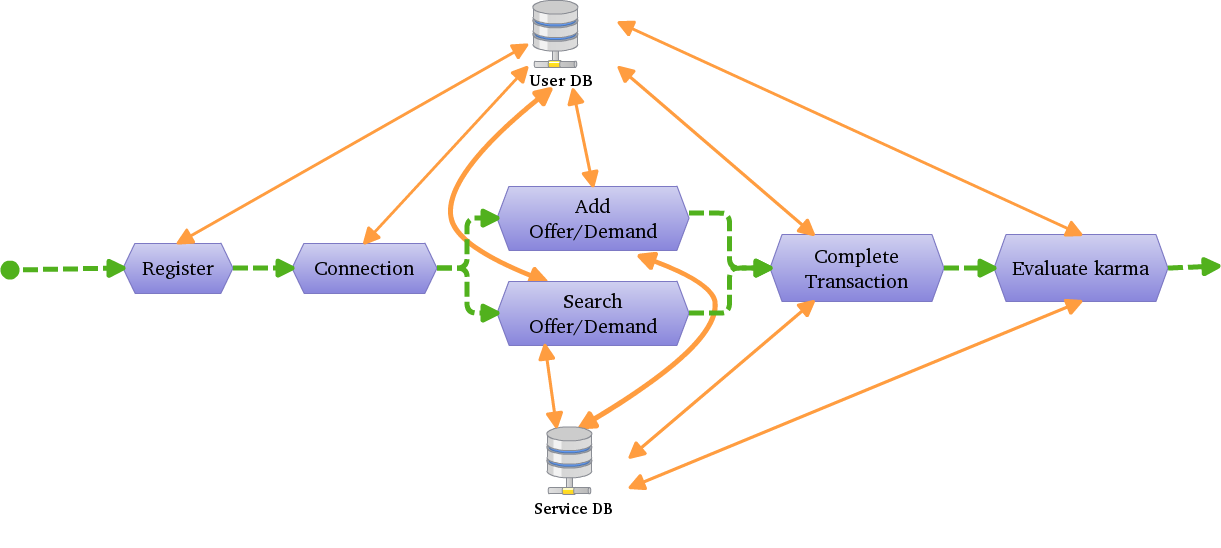
\includegraphics[width=.9\textwidth]{boxpointer.png}
		\caption{Box pointer diagram : Overall architecture}
		\label{fig:overall}
	\end{center}
\end{figure}

Even if the diagram shows two databases icons, there is currently only one (we can separate tables later if needed). The objective of the diagram is to know which datas are used by an operation. The user database means all people using the application (organisation co-workers, clients, etc.). Register and connection operations are both connected to an organisation or a standard user.


\subsection{Modelling part} %% TODO: another title...

\subsubsection{Class Diagram} %% TODO: another title...
\label{uml}
The diagram is available on the appendix, figure \vref{fig:uml}.\\
The class diagram shows the main classes of the model. Each variable of the class are detailed but only the main specific function that should be implemented are there. Also, note that to avoid overloading the diagram we didn't list all the getters and setters for the variables. The hollow arrow shows the extended classes. For example, the classes \texttt{Client} and \texttt{CoWorker} extend \texttt{User}. The simple arrow shows a link between two classes and the indexes the number of this object that can be own by the class. For instance, the link between \texttt{Address} and \texttt{User} means that a user can have many addresses (a star is used to denote that the number can be any), but an organisation can have only one address.\\

Looking at the diagram, we can see some classes extending \texttt{Abstract User}. There is \texttt{Client}, \texttt{Coworker} and \texttt{Moderator} (extended by \texttt{Admin}). This is due to the fact that they are all users but with specific rights on the website. There is also the explicit link showing that a coworker of an organisation manages multiple client profiles. On the centre, we have moderators that are linked with the services categories. Another interesting part of the diagram is the architecture of the \texttt{Offer} and \texttt{Demand}. Each of these two objects are extending the \texttt{Service} abstract class and are linked with a transaction. The transaction is the conclusion of a matching.\\

The UML Class Diagram would not have been completed if we had not included the \texttt{Database}, the \texttt{Controller} and the \texttt{View}. But at this stage of development it's too early to know their content. By too early we mean that we don't know yet how it will be implemented in our framework (RoR, more details on section \vref{ror}). Rather than listing a wrong list of methods and variables we decided to let them empty for the moment.


\subsubsection{Sequences Diagrams} %% TODO: another title...

\paragraph{Acceptance of an offer or a demand}

\begin{figure}[H]
	\begin{center}
		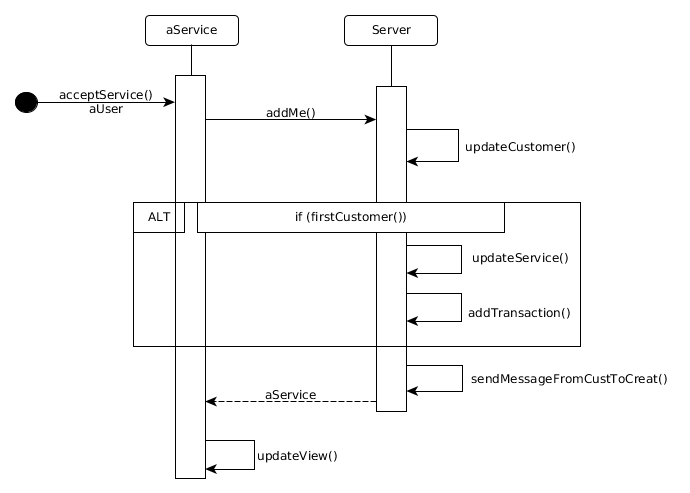
\includegraphics[width=.9\textwidth]{seq_acceptService.png}
		\caption{Sequence Diagram : Acceptance of an offer or a demand}
		\label{fig:acceptService}
	\end{center}
\end{figure}

The diagram on figure \vref{fig:acceptService} shows what happens when a user is interested by a service. First the user click on the 'Accept' button of this service (\texttt{aService} in the figure \ref{fig:acceptService}), then we add this user in the list of users interested in this service.
\\ 
We send a message from the customer to the creator to let him know his 
interest. We do this because we want to let the creator know about all the 
followers. It can be interesting, for example, if the first customer of the 
list didn't manifest after a long time or if the creator wants to know more
about the user.
\\
Each time a user accept the service, a confirmation demand is sent to the user that 
post the service. The user has to accept (or decline) and then the server do a 
transaction, update the service then we add this transaction to the 
"\textit{transactions historic}" of both the user and the creator of this service.


\paragraph{Creation of an offer or a demand}

\begin{figure}[H]
	\begin{center}
		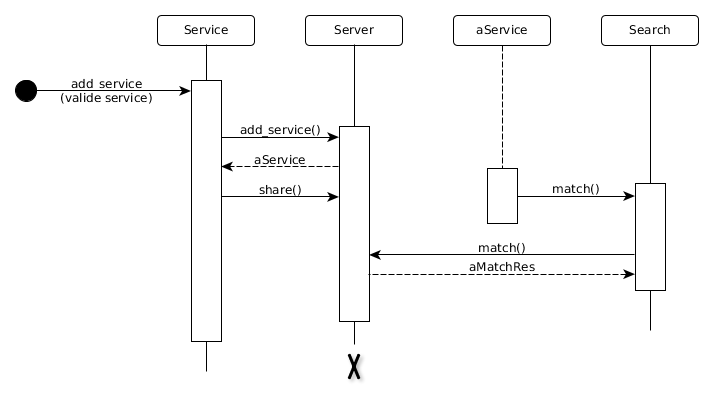
\includegraphics[width=.9\textwidth]{seq_addService.png}
		\caption{Sequence Diagram : Creation of an offer or a demand}
		\label{fig:addService}
	\end{center}
\end{figure}

The diagram on figure \vref{fig:addService} shows what happens when a user creates a service (an offer or a demand). After fulfilling the form and checking the integrity of the form, we send to the server the date, the server will then send an object service (\texttt{aService} in the figure \ref{fig:addService}). Then we give to the creator the opportunity of sharing this service with an eventual group and/or on a social network.\\
Meanwhile, we will do an automatic search to see if there is already an offer/demand in the database that can match this new service and show the results to the creator.

\paragraph{Creation of an account on the website}

\begin{figure}[H]
	\begin{center}
		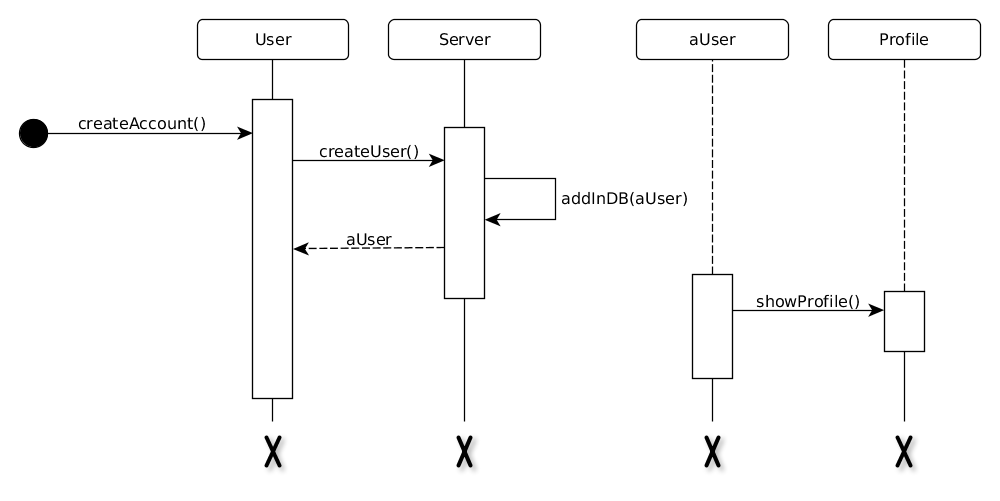
\includegraphics[width=.9\textwidth]{seq_createUser.png}
		\caption{Sequence Diagram : Creation of an account on the website}
		\label{fig:createUser}
	\end{center}
\end{figure}

In the figure \vref{fig:createUser}, we show the creation of a user account on the website. An unregistered user, after fulfilling the form and after having checked its integrity, will click the "\textit{Create Account}" button. We send the data from the form to the server, then the server adds this new user to the DataBase.\\
Then, it sends back a "\textit{user object}", an object which contains all the information that the user gives us plus his ID. With this information, we can show the \texttt{Profile} of the user.

\paragraph{The procedure of a search}

\begin{figure}[H]
	\begin{center}
		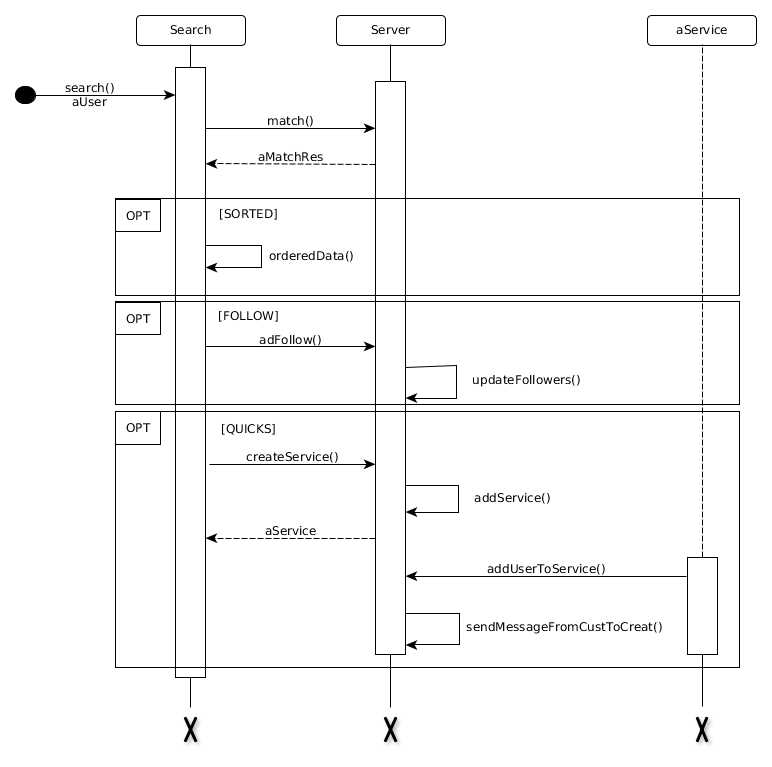
\includegraphics[width=.95\textwidth]{seq_search.png}
		\caption{Sequence Diagram : The procedure of a search}
		\label{fig:search}
	\end{center}
\end{figure}

In the figure \vref{fig:search}, we show the possibilities given to the user when he performs a search. After taking the data from the search form, the server performs a match and sends back the results.
Once we have the results, we can do several things.
\begin{itemize}
	\item \textsc{SORTED} : With this action, the user can order the results by different fields (date, creator, title, tag, ...)  in a decreasing or increasing order. We order in a dynamic way in this way we have less request on the server.
    \item \textsc{FOLLOW} : With this action, the user can add himself in the list of the followers of this service. A follower is always informed of the modifications on the service.
    \item \textsc{QUICKS} : With this action, the user can accept a service.  In our server, we perform this action by adding a new service that match with the request of the user.  After that, we perform the same actions that we explain in figure \vref{fig:acceptService}.
\end{itemize}

\paragraph{End of a Service, Evaluation and Karma}

\begin{figure}[H]
	\begin{center}
		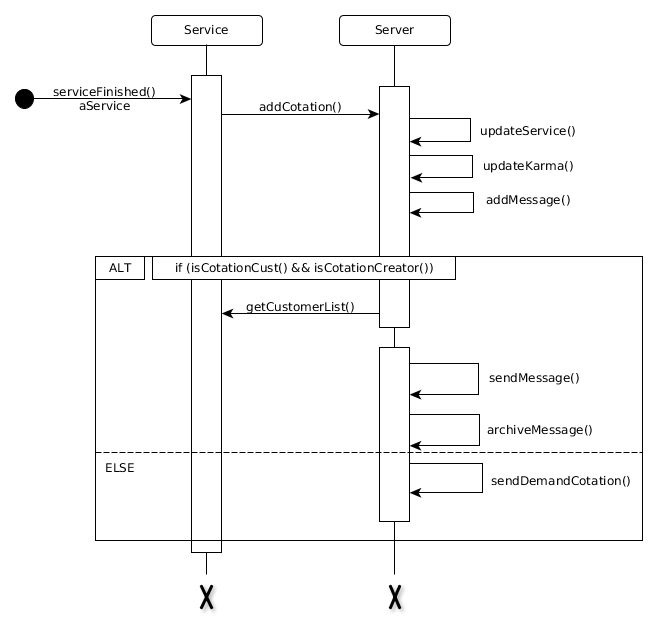
\includegraphics[width=.9\textwidth]{seq_serviceFinished.png}
		\caption{Sequence Diagram : End of a Service, Cotation and Karma}
		\label{fig:serviceFinished}
	\end{center}
\end{figure}

On the figure \vref{fig:serviceFinished}, we show what happens when a service is finished, i.e. when the customer and the creator met and performed the service.
\\ When it's finished, the creator and/or the customer can send a quotation with a optional message. 
\\ We get this informations from a form, the server then update the service, add karma (i.e. the quotation) to the customer or the creator and add the message to the 'transactions history' of the customer or creator.
\\ If the customer and the creator have given a evaluation, we ask to server the list of all other user interested by the service and send them a message to warn them that the offer/demand is not available anymore. After that, we archive the service.
\\ If the customer or the creator didn't give a evaluation, we send them a message and ask them to give one as soon as possible.


\subsection{Physical Architectural View}
Our physical architecture diagram is visible in the appendix: figure \vref{fig:physical_arch}.

\subsubsection{User's browser}
User's browser may run some JavaScript for loading some views, for example: sorting table or dynamically charge content like infinite scroll.

\subsubsection{RESTful web service}
With RoR, we can easily create RESTful web services thanks to Active Record. This is useful if Solidare-IT want to create a mobile application or a desktop application. The application will send requests to the server and the server will respond with JSON or XML structure.

\subsubsection{Production}
It's quite easy to switch between modules with Ruby: we can have a small environment for the development and a larger one for the production.\\
For the development part, we can have on the same machine a small webserver with WEBrick and a small database with SQLite.\\
On the other hand, for the production, we can use a more powerful webserver which can also be balanced on several machines. Instead of using SQLite, we can easily switch to PostgreSQL on separated machines just by modifying a configuration file.

%– A physical architectural view of your software which describes how the logical architectural view is mapped to the physical components and connectors on your implementation platform (for example, different processors and other devices)



\subsection{Pattern}
%– If applicable, a particular architectural style or pattern that is used. For example, it may be the case that the chosen web application framework imposes the use of a certain architectural pattern or architectural style (such as the model-view-controller architecture or MVC).

Ruby on Rails forces us to use the Model-View-Controller architectural style. Moreover, we all have experience with the MVC, then we will be more comfortable to code with this architecture.

\subsection{Testing our application}
Ruby gives us a lot of ways to test our application. We can easily generate test cases and use existing tools (CI: \textit{Continuous Integration}) to check if dependences need to be updated, the current build status, if the test cases are completed faster than before, etc.